\iffalse
  \author{EE24BTECH11032}
  \section{me}
  \chapter{2008}
\fi
\item $F\brak{z}$ is a function of the complex variable $z=x+iy$ given by $F\brak{z}=iz+kRe\brak{z}+iIm\brak{z}$.For what value of k will $F\brak{z}$ satisfy the Cauchy-Rienmann equations?
    \begin{enumerate}
        \item $0$
        \item $1$
        \item $-1$
        \item $y$
    \end{enumerate}
    \item A bar of uniform cross section and weighing $100$N is held horizontally using two massless and inextensible strings S1 and S2 as shown in the figure.\\
    %\begin{figure}[!ht]
\centering
\resizebox{3cm}{3cm}{%
\begin{circuitikz}
\tikzstyle{every node}=[font=\small]
\draw [<->, >=Stealth] (6.5,10.75) -- (6.5,8.25);
\draw [<->, >=Stealth] (5.25,9.25) -- (7.75,9.25);
\draw [<->, >=Stealth] (5.5,8.5) -- (7.5,10);
\draw [<->, >=Stealth] (5.5,10.25) -- (7.25,8.5);
\draw [<->, >=Stealth] (7,8.25) -- (6,10.5);
\draw [<->, >=Stealth] (5.25,9.75) -- (7.75,8.75);
\draw [<->, >=Stealth] (6,8.25) -- (7,10.5);
\draw [dashed] (3.25,9.25) -- (5.25,9.25);
\draw [dashed] (7.75,9.25) -- (8.75,9.25);
\draw [dashed] (6.5,10.5) -- (6.5,11.25);
\draw [->, >=Stealth] (6.5,11) -- (6.5,12.75);
\draw [->, >=Stealth] (8.75,9.25) -- (10.5,9.25);
\draw [dashed] (5.5,10.25) -- (3.75,11.75);
\draw [->, >=Stealth] (2.5,12.5) -- (3.25,11.75);
\draw [->, >=Stealth] (2.75,12.75) -- (3.5,12);
\draw [->, >=Stealth] (3,13) -- (3.75,12.25);
\draw [->, >=Stealth] (2.25,12.25) -- (3,11.5);
\node [font=\Huge] at (6.5,9.5) {.};
\node [font=\small] at (6.5,13) {$y$};
\node [font=\small] at (10.75,9.25) {$x$};
\node [font=\small] at (4.75,10) {$30\degree$};
\node [font=\small] at (4.25,12) {$U=1\;\frac{cm}{s}$};
\end{circuitikz}
}%
\end{figure}

    \begin{circuitikz}
\tikzstyle{every node}=[font=\large]
%\draw[fill={rgb,255:red,255; green,255; blue,255}] (2.5,16.75) rectangle (19,7);
\draw (3.5,14.75) to[short] (18,14.75);
\node [font=\Large] at (5.5,12.25) {$T_1$=?};
\node [font=\Large] at (11.25,12.25) {$T_2$=?};
\node [font=\Large] at (5.25,10.5) {S1};
\node [font=\Large] at (11.25,10.5) {S2};
\node [font=\Large] at (16,10.25) {Bar};
\draw [<->, >=Stealth] (4.5,8.5) -- (10.5,8.5);
\draw [<->, >=Stealth] (10.5,8.5) -- (16.75,8.5);
\node [font=\Large] at (9.5,15.75) {Rigid support};
\draw [short] (4.25,14.75) -- (4.5,15.25);
\draw [short] (4.75,14.75) -- (5,15.25);
\draw [short] (5.25,14.75) -- (5.5,15.25);
\draw [short] (5.75,14.75) -- (6,15.25);
\draw [short] (6.25,14.75) -- (6.5,15.25);
\draw [short] (6.75,14.75) -- (7,15.25);
\draw [short] (7.25,14.75) -- (7.5,15.25);
\draw [short] (7.75,14.75) -- (8,15.25);
\draw [short] (8.25,14.75) -- (8.5,15.25);
\draw [short] (8.75,14.75) -- (9,15.25);
\draw [short] (9.25,14.75) -- (9.5,15.25);
\draw [short] (9.75,14.75) -- (10,15.25);
\draw [short] (10.25,14.75) -- (10.5,15.25);
\draw [short] (10.75,14.75) -- (11,15.25);
\draw [short] (11.25,14.75) -- (11.5,15.25);
\draw [short] (11.75,14.75) -- (12,15.25);
\draw [short] (12.25,14.75) -- (12.5,15.25);
\draw [short] (12.75,14.75) -- (13,15.25);
\draw [short] (13.25,14.75) -- (13.5,15.25);
\draw [short] (13.75,14.75) -- (14,15.25);
\draw [short] (14.25,14.75) -- (14.5,15.25);
\draw [short] (14.75,14.75) -- (15,15.25);
\draw [short] (15.25,14.75) -- (15.5,15.25);
\draw [short] (15.75,14.75) -- (16,15.25);
\draw [short] (16.25,14.75) -- (16.5,15.25);
\draw [short] (16.75,14.75) -- (17,15.25);
\draw [fill={rgb,255:red,154; green,153; blue,150}] (4.5,9.75) rectangle (16.75,9);
\draw [short] (4.5,14.75) -- (4.5,9.5);
\draw [short] (10.5,9.75) -- (10.5,14.75);
\draw [->, >=Stealth] (4.5,9.75) -- (4.5,12.75);
\draw [->, >=Stealth] (10.5,9.75) -- (10.5,12.75);
\node [font=\LARGE] at (7.25,8) {L/2};
\node [font=\LARGE] at (13.75,8) {L/2};
\end{circuitikz}
    \begin{enumerate}
        \item $T_1=100N$ and $T_2=0N$
        \item $T_1=0N$ and $T_2=100N$
        \item $T_1=75N$ and $T_2=25N$
        \item $T_1=25N$ and $T_2=75N$
    \end{enumerate}
    \item If $\sigma_1$ and $\sigma_2$ are the algebraically largest and smallest principal stresses respectively, the value of the maximum shear stress is
    \begin{enumerate}
        \item $\frac{\sigma_1+\sigma_3}{2}$
        \item $\frac{\sigma_1-\sigma_3}{2}$
        \item $\sqrt{\frac{\sigma_1+\sigma_3}{2}}$
        \item $\sqrt{\frac{\sigma_1-\sigma_3}{2}}$
    \end{enumerate}
    \item The equation of motion for a spring-mass system excited by a harmonic force is $M\Ddot{x}+Kx=F\cos{\omega t}$, where the M is the mass, K is the spring stiffness, F is the force amplitude and $\omega$ is the angular frequency of excitation. Resonance occurs when $\omega$ is equal to 
    \begin{enumerate}
        \item $\sqrt{\frac{M}{K}}$
        \item $\frac{1}{2\pi}\sqrt{\frac{K}{M}}$
        \item $2\pi\sqrt{\frac{K}{M}}$
        \item $\sqrt{\frac{K}{M}}$
    \end{enumerate}
    \item For an Oldham coupling used between two shafts, which among the following statements are correct?\\
    A.\quad Torsional load is transferred along the shaft axis.\\
    B. \quad A velocity ratio of $1:2$ between shafts is obtained without using gears\\
    C. \quad Bending load is transferred transverse to shaft axis.\\
    D. \quad Rotation is transferred along the shaft axis.
    \begin{enumerate}
        \item A and C
        \item A and D
        \item B and C
        \item B and D
    \end{enumerate}
    \item For a two dimensional incompressible flow field given by $\vec{u}=A\brak{x\hat{i}-y\hat{j}}$, where $A>0$, which one of the following statements is FALSE?
    \begin{enumerate}
        \item It satisfies continuity equation.
        \item It is unidirectional when $x \to 0$ and $y \to \infty$.
        \item Its streamlines are given by $x=y$.
        \item It is irrotational.
    \end{enumerate}
    \item Which one of the following statements is correct for superheated vapour?
    \begin{enumerate}
        \item Its pressure is less than the saturation pressure at a given temperature.
        \item Its temperature is less than the saturation temperature at a given pressure.
        \item Its volume is less than the volume of the saturated vapour at a given temperature.
        \item Its enthalpy is less than the enthalpy of the saturated vapour at a given pressure.
    \end{enumerate}
    \item In a linearly hardening plastic material, the true stress beyond initial yielding 
    \begin{enumerate}
        \item increases linearly with the true strain
        \item decreases linearly with the true strain
        \item first increases linearly and then decreases linearly with the true strain
        \item remains constant
    \end{enumerate}
    \item The type of weld represented by the shaded region in the figure is \\ 
    %\begin{center}
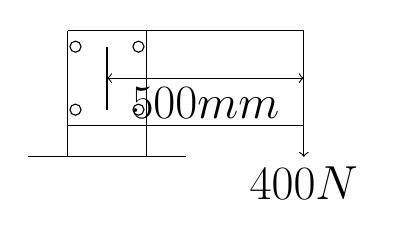
\begin{tikzpicture}
    % Draw rivets as circles
    \draw (0.4, 0.4) circle (2pt) node[above right] {};
    \draw (0.4, -0.4) circle (2pt) node[below right] {};
    \draw (-0.4, 0.4) circle (2pt) node[above left] {};
    \draw (-0.4, -0.4) circle (2pt) node[below left] {};

    

    % Draw horizontal and vertical distances between rivets
    \draw (0.5, 0.6) -- (-0.5, 0.6) ;
    \draw (0.5, -0.6) -- (-0.5, -0.6);
    \draw (-0.5, -0.6) -- (-0.5,0.6);
    \draw (0.5, -0.6) -- (0.5, 0.6);
    \draw (0.5, -0.6) -- (0.5, -1);
    \draw (-0.5, -0.6) -- (-0.5, -1);
   \draw (1, -1) -- (-1, -1);
    \draw (0.5, 0.6) -- (2.5, 0.6) ;
    \draw (0.5, -0.6) -- (2.5, -0.6) ;
    \draw (2.5 ,0.6) -- (2.5 ,-0.6);
    \draw[->] (2.5,-0.6) -- (2.5 ,-1) node[below]{$400N$} ;
    \draw (0,0.4) -- (0,-0.4);
    \draw[<->] (0,0) -- (2.5,0) node[below,midway]{$500 mm$};
\end{tikzpicture}
\end{center}

    \begin{circuitikz}
\tikzstyle{every node}=[font=\LARGE]

% Draw rectangles
\draw  (7.5,11.25) rectangle (8.25,6.75);
\draw  (5.5,6.75) rectangle (10.25,6);

% Draw the triangle and fill it
\fill[gray!30] (8.25,7.5) -- (9,6.75) -- (8.25,6.75) -- cycle; % Shaded triangle
\draw (8.25,7.5) -- (9,6.75);
\draw (9,6.75) -- (8.25,6.75);

\end{circuitikz}
    \begin{enumerate}
        \item groove
        \item spot
        \item fillet
        \item plug
    \end{enumerate}
    \item Using the Taylor's tool life equation with exponent $n=0.5$, if the cutting speed is reduced by $50$, the ratio of new tool life to original tool life to original tool life is 
    \begin{enumerate}
        \item $4$
        \item $2$
        \item $1$
        \item $0.5$
    \end{enumerate}
    \item A grinding ratio of $200$ implies that the 
    \begin{enumerate}
        \item grinding wheel wears $200$ times the volume of the material removed
        \item grinding wheel wears $0.005$ times the volume of the material removed
        \item aspect ratio of abrasive particles used in the grinding wheel is $200$
        \item ratio of volume of abrasive particle to that of grinding wheel is $200$
    \end{enumerate}
    \item Interpolator in a CNC machine
    \begin{enumerate}
        \item controls spindle speed
        \item coordinates axes movements
        \item operates tool changer
        \item commands canned cycle
    \end{enumerate}
    \item The time series forecasting method that gives equal weightage to each of the $m$ most recent observations is 
    \begin{enumerate}
        \item Moving average method
        \item Exponential smoothing with linear trend
        \item Triple Exponential smoothing 
        \item Kalman Filter
    \end{enumerate}
